\subsection{Bayer filter}
To capture color images conventional cameras use \glspl{cfa}.
The most common type of \gls{cfa} is the Bayer pattern where green pixels cover half the array in a lattice, and the red and blue pixel locations are spaced between the green pixels as shown in Figure \ref{fig:bayer_pattern} \cite{getreuerMalvarHeCutlerLinearImage2011}.
Different orderings of the colors in the \gls{cfa} exists, with the most common ones being RGGB, BGGR, GRBG, and GBRG where the letters designate the order of the four top left pixeld in the image.

\begin{figure}[H]
    \centering
    \begin{tabular}[b]{ccc}
        \subcaptionbox{RGGB bayer pattern}{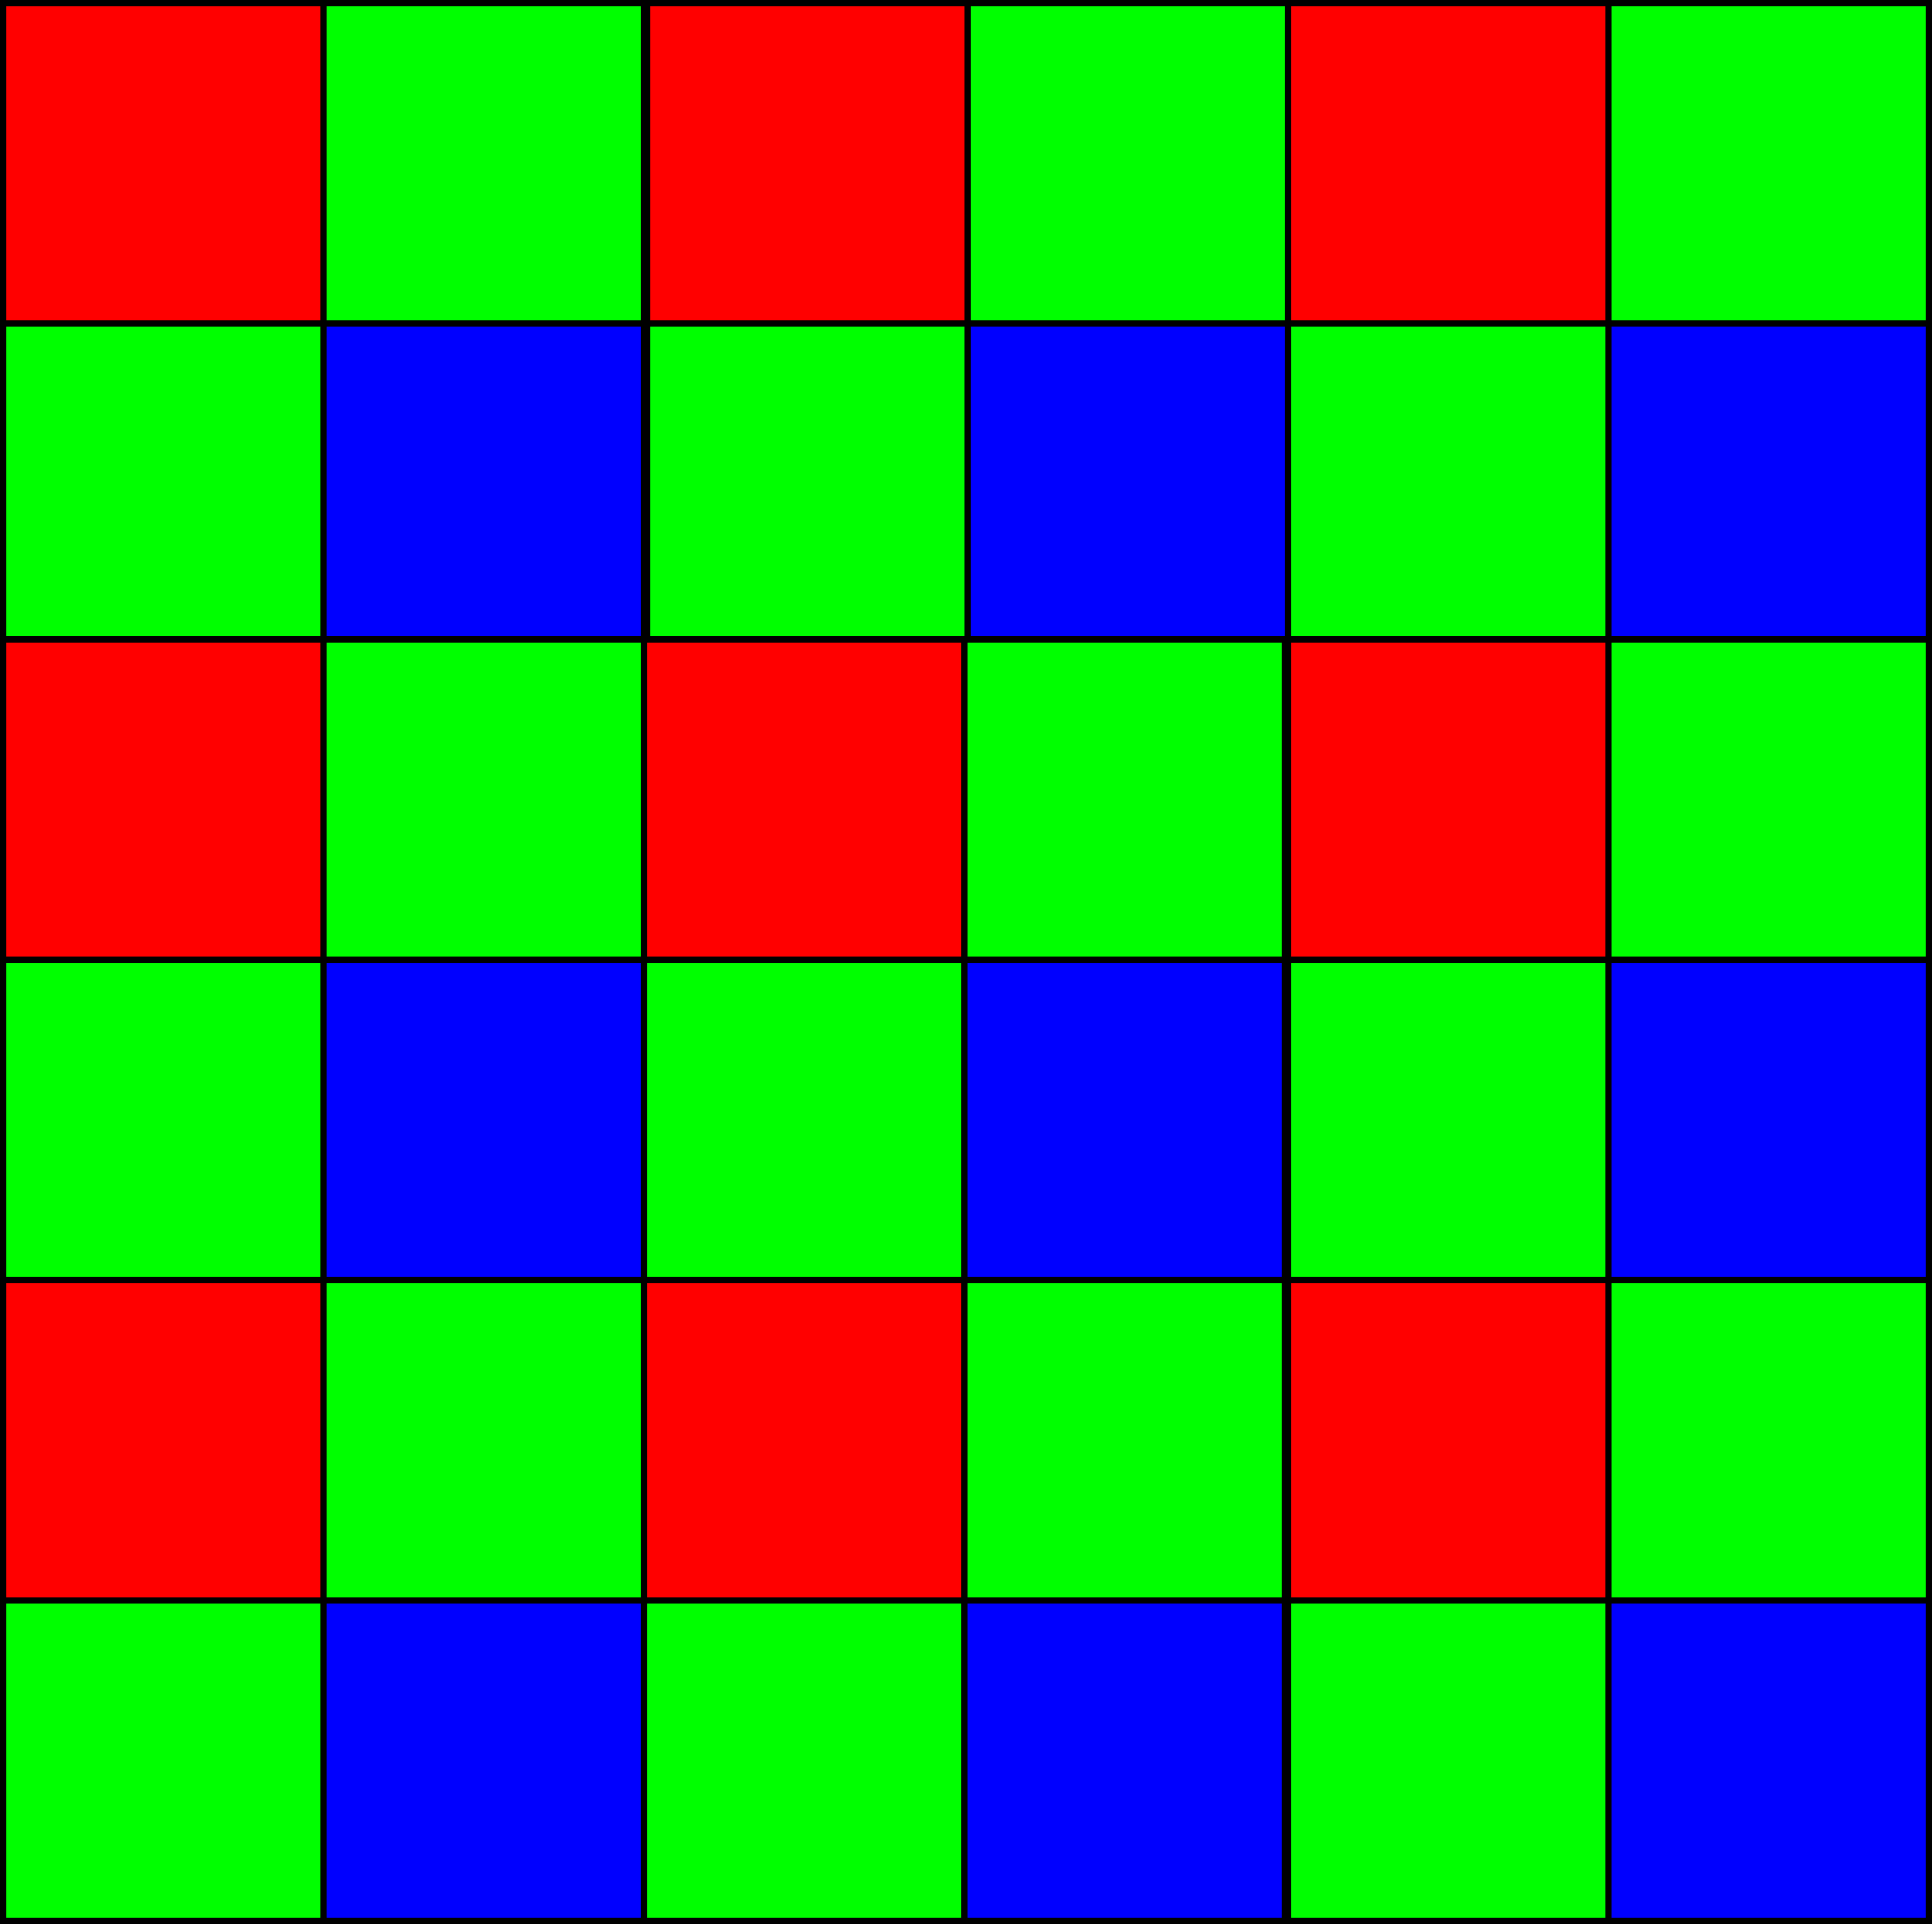
\includegraphics[width=0.25\textwidth]{figures/debayer/bayer_pattern.pdf}
            \label{fig:bayer_pattern}
        }                                                                                                              &
        \subcaptionbox{Green at red}{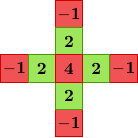
\includegraphics[width=0.25\linewidth]{figures/debayer/g_at_r.png}}               &
        \subcaptionbox{Green at red}{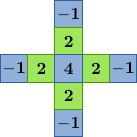
\includegraphics[width=0.25\textwidth]{figures/debayer/g_at_b.png}}                 \\
        \subcaptionbox{Red at }{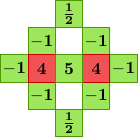
\includegraphics[width=0.25\textwidth]{figures/debayer/r_at_g_rr.png}}                 &
        \subcaptionbox{Red at green, blue row}{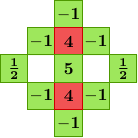
\includegraphics[width=0.25\textwidth]{figures/debayer/r_at_g_br.png}}  &
        \subcaptionbox{Red at blue}{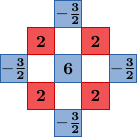
\includegraphics[width=0.25\textwidth]{figures/debayer/r_at_b.png}}                  \\
        \subcaptionbox{Blue at green, red row}{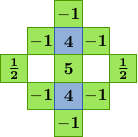
\includegraphics[width=0.25\textwidth]{figures/debayer/b_at_g_rr.png}}  &
        \subcaptionbox{Blue at green, blue row}{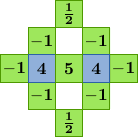
\includegraphics[width=0.25\textwidth]{figures/debayer/b_at_g_br.png}} &
        \subcaptionbox{Blue at red}{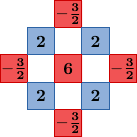
\includegraphics[width=0.25\textwidth]{figures/debayer/b_at_r.png}}
    \end{tabular}
    \caption{Bayer pattern and coefficient values used by Malvar-He-Cutler scaled by 8 \cite{getreuerMalvarHeCutlerLinearImage2011}\cite{CommonsBayerPattern2020}}
    \label{fig:debayer:malvar_filters}
\end{figure}

\subsection{Image demosaicing}
Image demosaicing is the process of estimating full-resolution color information for an image that has been captured with a bayer pattern \cite{liImageDemosaicingSystematic2008}, e.g. at each red pixel in the \gls{cfa} the green and blue intensities needs to be estimated.
Simple methods, such nearest neighbours or linear interpolation, are prone to yielding images false colors and the checkboard like patterns called the zipper effect as shown in Figure \ref{fig:artifacts_gioia} \cite{gioiaDataDrivenConvolutionalModel2021} \cite{liImageDemosaicingSystematic2008}.
A multitude of more advanced methods have been proposed with increasing sofisication and performance \cite{liImageDemosaicingSystematic2008}.
Lately different deep learning methods has also proven to perform very well at this task \cite{kwanComparisonDeepLearning2019}.

\begin{figure}[H]
    \centering
    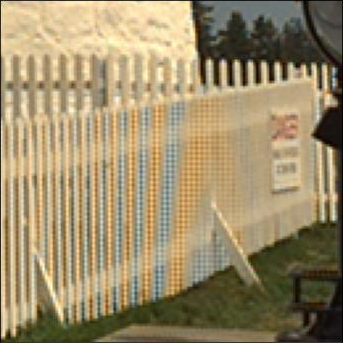
\includegraphics[width=0.5\textwidth]{figures/debayer/artifacts_gioia.png}
    \caption{Zipper effect and false colors \cite{gioiaDataDrivenConvolutionalModel2021}}
    \label{fig:artifacts_gioioa}
\end{figure}

\subsection{Malvar-He-Cutler}
\gls{mhc} pattented a simple but performant linear method using 5x5 filters that shows surprisingly good results \cite{malvarHighqualityGradientcorrectedLinear2009}.
The method they present is derived as a modification of bilinear interpolation, and it involves adding Laplacian cross-channel corrections to improve the quality of the bilinear method \cite{getreuerMalvarHeCutlerLinearImage2011}.
The demosaicking is implemented by convolution with a set of linear filters, and there are eight different filters for interpolating the different color components at different locations as can be shown in Figure \ref{fig:debayer:malvar_filters}.
Although several more sophisticated methods have been developed, the simple \gls{mhc} method works remarkably well \cite{liImageDemosaicingSystematic2008}\cite{kwanComparisonDeepLearning2019}\cite{getreuerMalvarHeCutlerLinearImage2011}.
The method is better suited for parallel execution than some others as discussed in \todo.



\subsection{Shortcomings}
A shortcoming of the current method is that it does not optimal gains.
Firstly the values used in \gls{mhc} are rounded to the neared dyadic rationals, to work efficently using integer arithmetic and bitshifting \cite{getreuerMalvarHeCutlerLinearImage2011}.
As the current proposed implementation uses floating point arithmetic, this rounding is disadventagious.
Another minor issues is that the values in \gls{mhc} were found to be the best fit for the well-known public-domain Kodak image set \cite{malvarHighqualityGradientcorrectedLinear2009}.
This is a set of 24 varied images, shown in Figure \ref{fig:kodak_image_suite}, that might not be the best representation of the images the \sr will capture in maritime environments.
It might be beneficial to recalculate the values based on a more representative dataset and use the floating point values rather than the rounded ones in the future.


\begin{figure}[H]
    \centering
    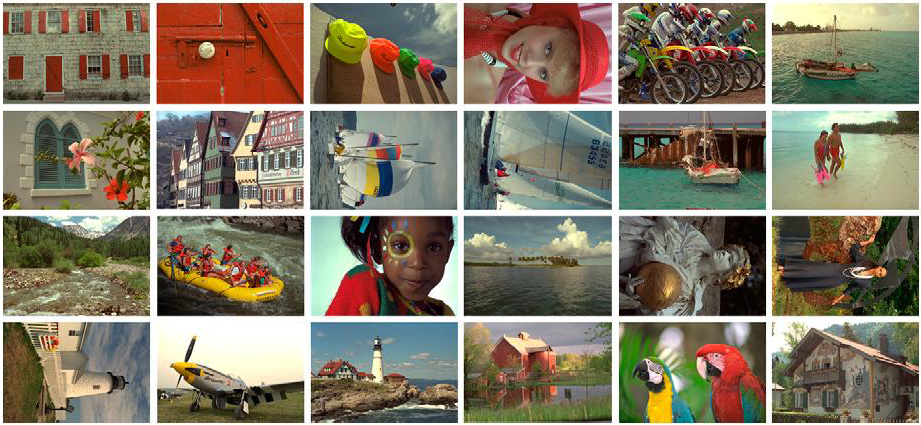
\includegraphics[width=0.8\textwidth]{figures/debayer/kodak_test_suite.png}
    \caption{Kodak image suite \cite{franzenTrueColorKodak2013}\cite{chungAdaptiveColorFilter2006}}
    \label{fig:kodak_image_suite}
\end{figure}


\begin{figure}[H]
    \centering
    \begin{tabular}[b]{ccc}
        \subcaptionbox{Exact image}{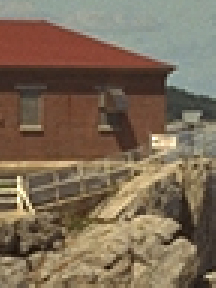
\includegraphics[width=0.3\textwidth]{figures/debayer/house_orig.jpg}}                           &
        \subcaptionbox{Observed Image}{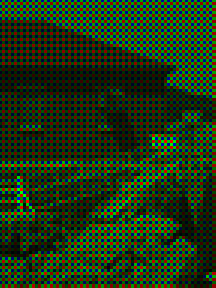
\includegraphics[width=0.3\textwidth]{figures/debayer/house_bayer.png}}                         \\
        \subcaptionbox{Bilinear (PSNR=25.61)}{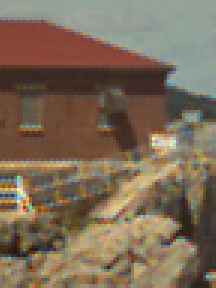
\includegraphics[width=0.3\textwidth]{figures/debayer/house_bilinear.png}}             &
        \subcaptionbox{Hamilton-Adams \todo (PSNR=31.62)}{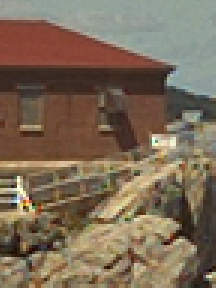
\includegraphics[width=0.3\textwidth]{figures/debayer/house_hamilton.png}} &
        \subcaptionbox{Malvar-He-Cutler (PSNR=31.15)}{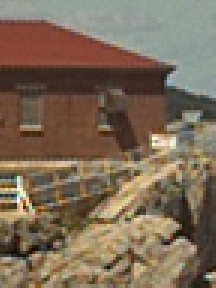
\includegraphics[width=0.3\textwidth]{figures/debayer/house_malvar.png}}
    \end{tabular}
    \caption{Coefficient values used by Malvar-He-Cutler scaled by 8 \cite{getreuerMalvarHeCutlerLinearImage2011}}
\end{figure}